\documentclass{article}
\usepackage{graphicx}
\usepackage{color}
\usepackage{fancyhdr}

\begin{document}



\title{\large{\textbf{PACT: \\ Programming $^{\wedge}$ Algorithms $\Longrightarrow$ Computational Thinking}}}

\author{PACT team at NUIM}

\begin{figure}
    \centering
    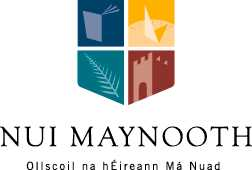
\includegraphics[width = 5cm]{nuim_large}
    \label{logo}
\end{figure}
\maketitle

\section{Introduction}
The PACT programme is a partnership between researchers in the department of Computer Science at the National University of Ireland Maynooth (NUIM) and teachers at selected post primary schools around the country. Initially the focus of this partnership is on teaching programming to transition year students, but ultimately the goal is to move beyond programming and algorithms towards computational thinking for the Junior Certificate cycle. Starting in September 2013 a number of Irish secondary schools commenced taking part in a pilot study of the new ``Computational Thinking" Transition Year module.

The team of researchers in NUIM who are involved are: 

\begin{itemize}
  \item Aidan Mooney
  \item James Power
  \item Rosemary Monahan
  \item Tom Naughton
  \item Susan Bergin
  \item Phil Maguire
  \item Joe Duffin
\end{itemize}

\section{Motivation}
Computational Thinking is about combining the creativity of human thinking with the power of computing machines to solve problems across a range of disciplines. It is a core skill which is crucial to many 21st century careers, not just in computer science, but also physics, finance, engineering and bioinformatics, to name a few. In addition to learning how to program in Python, Transition Year students taking this module learn how to apply their knowledge to model real-world problems. The focus of the module is not on learning facts about computers but on developing creative ideas and new ways of thinking.

The Computer Science department in NUIM, which recently celebrated its 25th anniversary, has collaborated with teachers across 9 secondary schools to develop a flexible module which will engage Transition Year students. Continuing feedback will be used to expand the module into a full Junior Cycle short course. 

\section{Background}
The Lero group in the University of Limerick are already working in the field of computer science education with Scratch-based material for primary and secondary schools. Lero support teachers, students, parents and schools in Scratch as well as creating extensive lesson plans and teaching material for schools \cite{scratch2013}.


Bridge21 is an education programme based in Trinity College which offer a new model of learning that can be adapted for use in secondary schools. They offer professional development workshops for teachers to train in certain areas \cite{bridge21}.

The Computing in Schools project in the United Kingdom looked at the current provision of education in Computing in UK schools, informed by evidence gathered from individuals and organisations with an interest in computing. One of their key findings was that the current delivery of Computing education in many UK schools is highly unsatisfactory. It also noted that there is a need to improve understanding in schools of the nature and scope of Computing. In particular there needs to be recognition that Computer Science is a rigorous academic discipline of great importance to the future careers of many pupils \cite{compSchools}.

\textbf{Need to put in more initiatives taking place around the world.}\\

\section{Experiment}
During the Summer of 2013 a number of schools were approached to gauge if there was interest in running such a pilot programme. The schools which came on board were:
\begin{itemize}
  \item Maynooth Post Primary School, Co. Kildare.
  \item Pobalscoil Neasain, Baldoyle, Dublin 13.
  \item Confey Community College, Leixlip, Co. Kildare.
  \item Castelcomer Community School, Co. Kilkenny.
  \item Scoil Mhuire Community School, Clane, Co. Kildare.
  \item Jesus and Mary College, Goatstown, Dublin 14.
  \item Salesian College, Celbridge, Co. Kildare.
\end{itemize}

At least one teacher from each of these schools agreed to participate in the pilot programme. The PACT team began to structure the content for the pilot programme and on the 25th of May and the 1st June 2013 two training sessions took place in NUIM. These sessions involved introducing the teachers to the content within the programme and also getting to know each other. It was hoped that a community of knowledge and learning would be created between all the teachers as they progressed with the pilot.

A Moodle system was hosted in the Department of Computer Science to store the content that was delivered in the training sessions. The content was divided in to five sections, namely:

\begin{enumerate}
  \item Introduction to Python I.
  \item Introduction to Python II.
  \item Algorithms.
  \item Graphics.
  \item Recursion and self-reference.
\end{enumerate}

Sections 1 and 2 provided an introduction to the Python programming language. These sections covered the basics of installation of Python and also looked at how to create and run programs written in Python. They looked at the main features of the language and gave sample programs for the teachers to use. An exercise book was created for all lessons within these sections which the teacher could use in class to get their students working in Python. In total 19 presentations were prepared for these sections which the teacher could break up into whatever format they felt worked for them. Section 3 focused on Algorithms and the process of writing them. It showed how to write a step by step procedure to solve particular problems. Section 4 looked at generating graphics using the Pygame set of modules. This section focused on allowing the participants to create fully featured games in the python language. Section 5 covers topics related to recursion which has been defined as ``the process of repeating items in a self-similar way" and is fundamental to the core theory of Computer Science. \\


\textbf{Should we put in learning outcomes here?}
\newline



Towards the end of the academic year 2013-14 we are going to host a competition which is open to all the students who were involved with the PACT pilot programme. This competition is aimed at providing examples of best practice and each school participating in the pilot is invited to select up to two teams, consisting of 3-5 students, to participate in the competition. The selection of teams and team members is entirely at the discretion of the schools. Participants in the competition should highlight explicitly how their experience with the PACT programme has contributed to two or more of the six key areas identified by the NCCA, namely:

\begin{enumerate}
  \item Managing Myself.
  \item Staying Well.
  \item Communicating.
  \item Being Creative.
  \item Working with Others.
  \item Managing Information and Thinking \cite{ncca2013}.
\end{enumerate}



\section{Future Work}
As of the 1st April 2014 we have already received interest from the following schools:
\begin{itemize}
  \item Tallaght Community School, Dublin. 
  \item Sandford Park, Ranelagh, Dublin.
  \item St. Munchin's College, Limerick.
  \item Beneavin college, Finglas, Dublin.
\end{itemize}

These schools have approached us directly from seeing our webpage or from teachers who are involved in the pilot programme this year. We hope to run this programme again for the academic year 2014-15 with a larger number of schools and take on board the feedback received from the teachers and students in the first year.

\section{Contact Us}
The PACT team can be contacted at the following email address: \textcolor{red}{pact@cs.nuim.ie}.
Our website is: \textcolor{red}{www.cs.nuim.ie/pact}.

\bibliographystyle{alpha}
\bibliography{ref}
\end{document}
